\chapter{Tensors and Multilinear Model}
\label{chap_mult_model}
\section{Tensor Notation}
% tensor notations

In this section we mostly follow Elden and Savas \cite{elden_savas_2009}, but the
definition of a mode-$k$ product is taken from  Kolda and Bader \cite{kolda_bader_2009}.


By tensors we mean multidimensional arrays, that is, sets of real numbers 
$ \X = \{\X_{i_1 i_2 \dots i_n} \} $ indexed by sets $1 \leq i_j \leq I_j$.
The number of dimensions $n$ is called the order of the tensor, such tensors 
are also called $n$-way tensors.
Sometimes it will be more convenient to use Matlab-like notation. For example, if we have a matrix $M \in R^{I_1 \times I_2}$ and $1 \leq a < b \leq I_1$, the submatrix
of $M$ obtained by 'cutting out' rows from $a$ to $b$ is denoted by $M(a:b, :)$. The meaning of 
 $M(:, c:d)$ and $M(a:b, c:d)$ is also clear (of course, $1 \leq c < d \leq I_2$).
 


The set of all tensors with fixed dimensions $I_1$, $I_2$, $I_3$ is denoted by 
${\R}^{I_1 \times I_2 \times I_3}$. It has a natural structure of a vector space
with the canonical inner product defined by
\begin{equation}
    \langle \A, \B \rangle = \sum_{i_1 = 1}^{I_1}  \sum_{i_2 = 1}^{I_2} \sum_{i_3 = 1}^{I_3}  \A_{i_1, i_2, i_3} \B_{i_1, i_2, i_3}.
\end{equation}
The norm of the tensor defined by this tensor product is called a Frobenius norm:
\begin{equation}
    \| \A \| = \sqrt{ \langle \A, \A \rangle }.
\end{equation}


Matrices can be considered as ordered sets of vectors in two natural ways: they have
rows and columns. In the same way, tensors of order $3$ have $I_2 I_3 $ mode-$1$ fibers which
are elements of $\R^{I_1}$, $I_1 I_3$ mode-$2$ fibers (vectors from $\R^{I_2}$), and $I_1 I_2$ mode-$3$
fibers (vectors from $\R^{I_3}$). This notion is illustrated in Figure \ref{fig: img_tensor_3}.


\begin{figure}[t!]
\centering
    \begin{subfigure}[b]{0.24\textwidth}
        \centering
        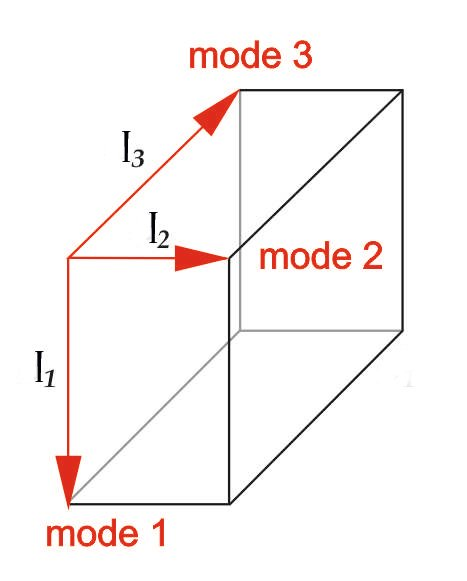
\includegraphics[height=1.3in]{images/tensor_3.jpg}
        \caption{}
    \end{subfigure}
    \begin{subfigure}[b]{0.24\textwidth}
        \centering
        
\includegraphics[height=1.3in]{images/fiber_1.jpg}
        \caption{}
    \end{subfigure}
    \begin{subfigure}[b]{0.24\textwidth}
        \centering
        
\includegraphics[height=1.3in]{images/fiber_2.jpg}
        \caption{}
    \end{subfigure}
    \begin{subfigure}[b]{0.24\textwidth}
        \centering
        
\includegraphics[height=1.3in]{images/fiber_3.jpg}
        \caption{}
    \end{subfigure}
    \caption{(a) A mode-$3$ tensor; (b) mode-1 fibers of a tensor; (c) mode-$2$ fibers of a tensor; (d) mode-$3$ fibers of a tensor.}
    \label{fig: img_tensor_3}
\end{figure}


Let $A$ be a $J \times I_1$ matrix $A$. If we multiply a mode-$1$ fiber of $\X \in \R^{I_1 \times I_2 \times I_3}$ by $A$,
we get a vector from $\R^J$. Doing this with every fiber, we get a new tensor from $\R^{J \times I_2 \times I_3}$. This is denoted by 
$\X \times _{1} A$ and called a mode-$1$ product of $\X$ and $A$. In the same way we define mode-$k$ product of a tensor and a matrix. Namely,
if $A \in \R^{J \times I_k}$, then $\X \times_k A$ is a tensor defined by
\begin{equation}
    (\X \times_k A)(i_1, \dots, i_{k-1}, j, i_{k+1}, \dots, i_n) = \sum_{i_k = 1}^{I_k} \X(i_1, \dots, i_n) A(j, i_k).
\end{equation}
This operation has the following properties:
\begin{enumerate}
\item The products in different modes commute:
\begin{equation}
n \not= m \Rightarrow (\A \times _n B) \times_m C = (\A \times _m C) \times_n B.
\end{equation}
\item The product in one mode is associative:
\begin{equation}
(\A \times_n B) \times_n C = \A \times_n (BC).
\end{equation}
\item Orthogonal factors preserve Frobenius norm:

\begin{equation}
\label{orthogonal_norm_inv}
S \in O(I_k)  \Rightarrow \| \A \times_k S \| = \| \A \|.
\end{equation}
\end{enumerate}

There is a natural way of transforming a tensor $\X \in R^{I_1 \times I_2 \times \cdots \times I_N}$ into a matrix: choose one mode $n$
and arrange all mode-$n$ fibers into a matrix in a natural order. More formally,
the unfolding in mode $n$ is an $I_n \times \prod_{k \neq n} I_k$ matrix such that
the element $X_{i_1 \dots i_N}$ is mapped to the row $i_n$ and column $j = 1 + \sum_{ k \neq n} (i_k - 1) J_k$,
with $J_k = \prod_{ m \in \{ 1, \dots, k-1 \} \\ {n} } I_m$.
 Unfolding  is a special case of \textit{matricization}. In general, in order to get a matrix
from $\X$ we fix the modes $\mathbf{r} =  (r_1, \dots, r_L)$ that will be mapped to rows.
Here $1 \leq r_i \leq n$ are distinct numbers. The other $M = n - L$  modes will be mapped
to columns $\mathbf{c} = (c_1, \dots, c_M)$.
The element $\X(j_1, \dots, j_n)$ is mapped to $X^{(\mathbf{r};\mathbf{c})}(j, k)$, where
\begin{eqnarray}
    j = 1 + \sum_{l = 1}^{L} ( i_{r_{L-l+1}} - 1) \prod_{l' = 1}^{l - 1} d_{r_{L - l' + 1}}, \\
    k = 1 + \sum_{m = 1}^{M} ( i_{r_{M-m+1}} - 1) \prod_{m' = 1}^{m - 1} d_{r_{M - m' + 1}}.
\end{eqnarray}
We illustrate the general formula with two specific examples
for a $4$-way tensor (we shall need these examples in Section \ref{sec_newgr}).

If $\X \in \R^{I_1 \times I_2 \times I_3 \times I_4}$, then $\X^{(1,3;2,4)}$ is a 
matrix with $I_1 I_3$ rows and $I_2 I_4$ columns obtained by the following rule:
an element $\X(i_1, i_2, i_3, i_4)$ goes to the row $i$, column $j$ of $\X^{(1,3;2,4)}$,
where 
\begin{eqnarray}
i = 1 + (i_3 - 1) + (i_1 -1) I_3 \\
j = 1 + (i_4 - 1) + (i_2 -1) I_4.
\end{eqnarray}
The order of indices in $\mathbf{r}$, $\mathbf{c}$ is significant: the second matricization
we shall need is $\X^{(1,3;4,2)}$. The formulas for this variant are
\begin{eqnarray}
i = 1 + (i_3 - 1) + (i_1 -1) I_3 \\
j = 1 + (i_2 - 1) + (i_4 -1) I_2 .
\end{eqnarray}



Let $\A \in \mathbb{R}^{I_1 \times \cdots \times I_k} $ and $\B  \in \mathbb{R}^{J_1 \times \cdots \times J_m}$ be tensors.
Their \textit{tensor product} is the tensor $ \A \otimes B  \in {\R}^{I_1 \times \cdots \times I_k \times J_1 \times \cdots \times J_m } $
defined by
\begin{equation}
    (\A \otimes B)(i_1, \dots, i_k, j_1, \dots, j_m) = \A(i_1, \dots, i_k) B(j_1, \dots, j_m).
\end{equation}
If $I_{\kappa} = J_{\mu}$, we define the \textit{contracted product} $\C = \langle \A, \B \rangle_{\kappa; \mu} $ of $\A$ and $\B$ in dimensions $\kappa$, $\mu$ as a tensor
obtained from $\A \otimes \B$ by 'summing out' in modes $I_{\kappa}$ and $J_{\mu}$, that is,
%\in {\R}^{I_1 \times \cdots I_{\kappa - 1} \times I_{\kappa +1} \times \cdots \times I_k \times J_1 \times  \cdots \times J_m } 
\begin{eqnarray}
    \C(i_1, \dots, i_{\kappa-1}, i_{\kappa + 1} , \dots, i_{k}, j_1, \dots, j_{\mu - 1}, j_{\mu+1}, \dots, j_{m}) = \notag\\
    \sum_{t = 1}^{I_{\kappa}} (\A \otimes \B)(i_1, \dots, i_{\kappa-1}, t, i_{\kappa+1}, \dots,  i_k, j_1, \dots, j_{\mu-1}, t, j_{\mu+1}, \dots, j_m).
\end{eqnarray}
If $I_{\kappa_1} = J_{\mu_1}$ and $I_{\kappa_2} = J_{\mu_2}$, then we can contract
by summing out in two pairs of modes in the same way. This contracted product is 
denoted by $\langle \A, \B \rangle_{\kappa_1, \kappa_2; \mu_1, \mu_2}$.



If $\A$ and $\B$ are of the same order ($k = m$), then the notation is more compact.
If $\kappa = \mu$, then the contracted product
$\langle \A, \B \rangle_{\kappa; \kappa}$
is denoted by $\langle \A, \B \rangle_{\kappa}$. Analogous notation $\langle \A, \B \rangle_{(\kappa_1, \kappa_2)}$ is equivalent to $\langle \A, \B \rangle_{(\kappa_1, \kappa_2;\kappa_1, \kappa_2)}$.
The minus in $\langle \A, \B \rangle _{ -(\kappa_1, \dots, -\kappa_p)}$ means 
that contraction is performed in all modes but $\kappa_1, \dots, \kappa_p$. The following examples 
illustrate these definitions.


If $\A, \B \in \R^{I_1 \times I_2 \times I_3 \times I_4}$, then
\begin{eqnarray*}
\begin{split}
\langle \A, \B \rangle_{(2,3)} & \in \R^{I_1 \times I_4 \times I_1 \times I_4} \\
\left( \langle \A, \B \rangle_{(2,3)}\right)(i_1, i_4, j_1, j_4) &= \sum_{i_2 = 1}^{I_2} \sum_{i_3 = 1}^{I_3} \A(i_1, i_2, i_3, i_4) \B(j_1, i_2, i_3, j_4) \\
\langle \A, \B \rangle_{-3)} &= \langle \A, \B \rangle_{(1,2,4))} \in \R^{I_3 \times I_3} \\
\left( \langle \A, \B \rangle_{-3)}\right)(i_3, j_3) &= \sum_{i_1 =1 }^{I_1} \sum_{i_2 = 1}^{I_2} \sum_{i_4 = 1}^{I_4} \A(i_1, i_2, i_3, i_4) \B(i_1, i_2, j_3, i_4) 
\end{split}
\end{eqnarray*}


\section{Tucker Decomposition}

The material of this section comes from Kolda and Bader \cite{kolda_bader_2009}.

Suppose that we want to compress a $3$-mode tensor: instead of $\A \in \R^{d_1 \times d_2 \times d_3}$
we want to store only $\G \in \R^{r_1 \times r_2 \times r_3}$, where $r_k \leq d_k$.
The compression is performed by applying projections to a lower-dimensional
space in each mode, so that
\begin{equation}
    \G = \A \times_1 F_1 \times_2 F_2 \times_3 F_3, \quad F_i \in \R^{r_i \times d_i}.
\end{equation}
Though it  is not necessary to impose any constraints on the  projection matrices $F_i$,
it is usually assumed that they have orthonormal columns. In this case it is
easy to restore the approximate version of $\A$ from $G$:
\begin{equation}
    \A \approx \G \times _{1} F_1^T \times _{2} F_2^T \times _{3} F_3^T.
\end{equation}
This approximation is called Tucker decomposition. It was introduced in Tucker \cite{tucker_63}.
As a side remark we notice that there is a specific case of Tucker decomposition
called CP. The minimal number of components (they are called \textit{rank-1 tensors}) needed
in CP decomposition to exactly represent $\A$ is called \textit{the rank of $\A$}, and
finding this rank is an NP-hard problem (\cite{tensor_rank_np_complete}, \cite{tensors_np_hard}).



We shall use a variant of Tucker decomposition (known as Tucker2)
in which we do not compress in mode $1$, so $F_1$ is fixed to be
the identity matrix.  
The Frobenius norm of the residual $\| \A - \G \times _{1} F^T_1 \times _{2} F^T _2 \times _{3} F^T_3 \|$ is a natural measure of the quality of approximation, 
so the best Tucker2 decomposition is a solution of
the following optimization problem:
\begin{equation}
    \label{tucker_min}
\| \A - \G \times_2 F_2^T \times_3 F_3^T \| \to \min
\end{equation}
where $F_2$ and $F_3$ are matrices with orthonormal columns.
The following equality holds (see Kolda and Bader \cite{kolda_bader_2009}, section 4.2, for the proof).
\begin{equation}
\label{tucker_min_max}
\begin{split}
    \| \A - \G \times_2 {F_2^T} \times_3 {F_3^T} \|^2  &= \| \A \|^2 - \| \G \|^2 \\
                                                       & = \| \A \|^2 - \| \A \times_2 {F_2} \times_3 {F_3} \|^2.
\end{split}
\end{equation}
In particular, this equality proves that the Frobenius norm
of the compressed version of $\A$ ('energy') cannot be greater than the norm
of the original tensor $\A$. It also shows that the best decomposition
is a solution of the maximization problem
\begin{equation}
\label{tucker_max}
\Phi(F_2, F_3) = \frac{1}{2} \| \A \times_2 F_2 \times_3 F_3 \|^2 \to \max.
\end{equation}
Since the set of matrices with orthonormal columns is bounded and closed,
this problem is guaranteed to have a solution by Weierstrass extreme value theorem.
Property \eqref{orthogonal_norm_inv} implies that
for all orthogonal matrices $S_2 \in O(d_2)$, $S_3 \in O(d_3)$
\begin{equation}
    \Phi(F_2 S_2, F_3 S_3) = \Phi(F_2, F_3),
\end{equation}
so the best Tucker2 decomposition is not unique. 
The geometric interpretation of this fact
is that we are actually looking for subspaces
the projection to which preserves as much energy
as possible, and the exact projection operators
given by the $F_i$ matrices do not matter, as they are 
just another choice of the basis in the same subspace.



We shall discuss methods of computing Tucker2 decomposition in Chapter \ref{chap_algo}.


\section{Multilinear Model}
\label{mult_model}

This thesis uses the multilinear model as it is formulated in Bolkart and Wuhrer \cite{bolkart_wuhrer_2013}. The model was first introduced by Vlasic et al. \cite{vlasic}.



Suppose that we have a set of registered and spatially aligned 3D face scans of different people expressing different emotions.
The registration process must ensure that all scans have the same number of points
and these points must be in dense correspondence to each other, otherwise
it would not make sense to apply statistical methods
to the data. It is also necessary to have full set of expressions for each 
person (we do not consider the problem of restoring missing data).



We can organize these data in a $3$-way tensor. Mode $1$ corresponds
to coordinates, mode $2$ is identity, and mode $3$ is expression.
To this end, we flatten each scan: if $(p_1, \dots, p_n)$ is a set of points in $\R^3$, then we write
the coordinates of all points into one vector $(p_{1, x}, p_{1, y}, p_{1, z}, \dots, p_{n, x}, p_{n, y}, p_{n, z}$
and take this vector as mode-$1$ fiber of the tensor $\Y$. The fibers $\Y(:, i, j)$
and $\Y(:, i', j)$ represent different persons with the same expression, the fibers
$\Y(:, i, j)$ and $\Y(:, i, j')$ are scans of the same person performing different expressions. 
The tensor $\Y$ has dimensions $d_1$, $d_2$, $d_3$, where $d_1 / 3$ is the number
of points in each scan, $d_2$ is the number of people, and $d_3$ is the number
of expressions. This arrangement is schematically depicted in Figure \ref{fig:img_mult_model}.



\begin{figure}[t!]
\centering
        
\includegraphics[height=1.6in]{images/mult_model.jpg}
    \caption{A scheme of modes in the multilinear model.}
    \label{fig:img_mult_model}
\end{figure}

The first step is to calculate the \textit{mean face} $\bmu$,
\begin{equation}
    \bmu := \frac{1}{d_2 d_3} \sum_{i_2, i_3} \Y(:, i_2, i_3).
\end{equation}
Then we subtract $\bmu$ from all mode-$1$ fibers and get a centered tensor $\A$, 
which is compressed using Tucker2 decomposition for some $r_2 < d_2$, $r_3 < d_3$,
\begin{equation}
    \A \approx \G \times_2 F_2^T \times_3 F_3^T.
\end{equation}



This is a generative model. If we choose $\mathbf{w}_2 \in \R^{r_2}$,
$\w_3 \in \R^{r_3}$, we can generate a new face as
\begin{equation}
    \label{mlm_generate}
    \f(\w_2, \w_3) = \bmu +  \G \times_2 \w_2 \times_3 \w_3
\end{equation}
The idea is that by changing $\w_2$ we should get a face of another person
with the same expression, by changing $\w_3$ we keep the identity
and change only the expression. Therefore $\w_2$ is called \textit{identity weights}
and $\w_3$ is called \textit{expression weights}.


Let $\tilde{\f}$ be some face scan. The problem of finding
identity and expression weights such that the corresponding face
$\f(\w_2, w_3)$ is a good approximation of $\tilde{\f}$ is
called  \textit{fitting}. It can be formulated as the following optimization problem:
\begin{equation}
\label{mult_model_fit}
\mbox{Find $\w_2 \in \R^{r_2}$, $\w_3 \in \R^{r_3}$ that minimize } \rho(\tilde{\f}, \bmu + \G \times_2 \w_2 \times_3 \w_3) \to \min.
\end{equation}
The identity and expression weights $\w_2$, $\w_3$ can be regarded as a compact low-dimensional
representation of $\tilde{\f}$. More details on  objective function $\rho$ 
will be given in Section \ref{eval_fit}.


As a final remark we note that this model is a generalization of Principal Component 
Analysis (PCA). In PCA we are looking for a subspace projection to which
preserves as much variation as possible, that is, we approximate
the (centered) data with a linear subspace.
In multilinear model we are looking for two subspaces and perform projection
in different modes. If we fix expression, the multilinear model
also gives us a linear (or, more precisely, an affine) subspace that approximates 
the set of faces with  this expression. Indeed,
the equation \eqref{mlm_generate} for fixed $\w_3$ is a parametric
equation of an affine subspace. However, when we change
expression, this subspace changes in a linear fashion. Of course,
expression and identity play symmetric roles.
